%%=============================================================================
%% LaTeX sjabloon voor bachelorproef, HoGent Bedrijf en Organisatie
%% Opleiding Toegepaste Informatica
%%=============================================================================

\documentclass[fleqn,a4paper,12pt]{book}

%%=============================================================================
%% LaTeX sjabloon voor de bachelorproef, HoGent Bedrijf en Organisatie
%% Opleiding toegepaste informatica
%%
%% Structuur en algemene vormgeving. Meestal hoef je hier niets te wijzigen.
%%
%% Vormgeving gebaseerd op "The Legrand Orange Book", version 2.0 (9/2/15)
%% door Mathias Legrand (legrand.mathias@gmail.com) met aanpassingen door
%% Vel (vel@latextemplates.com). Het oorspronkelijke template is te vinden op
%% http://www.LaTeXTemplates.com
%%
%% Aanpassingen voor HoGent toegepaste informatica: 
%%   Bert Van Vreckem <bert.vanvreckem@hogent.be>
%% Licentie: 
%%   CC BY-NC-SA 3.0 (http://creativecommons.org/licenses/by-nc-sa/3.0/)
%%=============================================================================

%%-----------------------------------------------------------------------------
%% Packages
%%-----------------------------------------------------------------------------

\usepackage[top=3cm,bottom=3cm,left=3cm,right=3cm,headsep=10pt,a4paper]{geometry} % Page margins
\usepackage[utf8]{inputenc}  % Accenten gebruiken in tekst (vb. é ipv \'e)
\usepackage{amsfonts}        % AMS math packages: extra wiskundige
\usepackage{amsmath}         %   symbolen (o.a. getallen-
\usepackage{amssymb}         %   verzamelingen N, R, Z, Q, etc.)
\usepackage[english,dutch]{babel}    % Taalinstellingen: woordsplitsingen,
                             %  commando's voor speciale karakters
                             %  ("dutch" voor NL)
\usepackage{iflang}
\usepackage{eurosym}         % Euro-symbool €
\usepackage{geometry}
\usepackage{graphicx}        % Invoegen van tekeningen
\graphicspath{{img/}}       % Specifies the directory where pictures are stored
\usepackage{tikz}            % Required for drawing custom shapes
\usepackage[pdftex,bookmarks=true]{hyperref}
                             % PDF krijgt klikbare links & verwijzingen,
                             %  inhoudstafel
\usepackage{enumitem}        % Customize lists
\setlist{nolistsep}         % Reduce spacing between list items
\usepackage{listings}        % Broncode mooi opmaken
\usepackage{multirow}        % Tekst over verschillende cellen in tabellen
\usepackage{rotating}        % Tabellen en figuren roteren

\usepackage{booktabs}        % Required for nicer horizontal rules in tables

\usepackage{xcolor}          % Required for specifying colors by name
\definecolor{maincolor}{RGB}{0,147,208} % Define the main color used for 
                             % highlighting throughout the book
                             % 0, 147, 208 = officiële kleur HoGent FBO

% Paragraph style: no indent, add space between paragraphs
\setlength{\parindent}{0em}
\setlength{\parskip}{1em}

\usepackage{etoolbox}
\usepackage{titling} % Macros for title, author, etc
\usepackage{lipsum}          % Voor vultekst (lorem ipsum)

%----------------------------------------------------------------------------------------
%	FONTS
%----------------------------------------------------------------------------------------

\usepackage{avant} % Use the Avantgarde font for headings
%\usepackage{times} % Use the Times font for headings
\usepackage{mathptmx} % Use the Adobe Times Roman as the default text font together with math symbols from the Sym­bol, Chancery and Com­puter Modern fonts

\usepackage{microtype} % Slightly tweak font spacing for aesthetics
\usepackage[utf8]{inputenc} % Required for including letters with accents
\usepackage[T1]{fontenc} % Use 8-bit encoding that has 256 glyphs

%------------------------------------------------------------------------------
%	TITLE PAGE
%------------------------------------------------------------------------------

\newcommand{\inserttitlepage}{%
\begin{titlepage}
  \newgeometry{top=2cm,bottom=1.5cm,left=1.5cm,right=1.5cm}
  \begin{center}

    \begingroup
    \rmfamily
    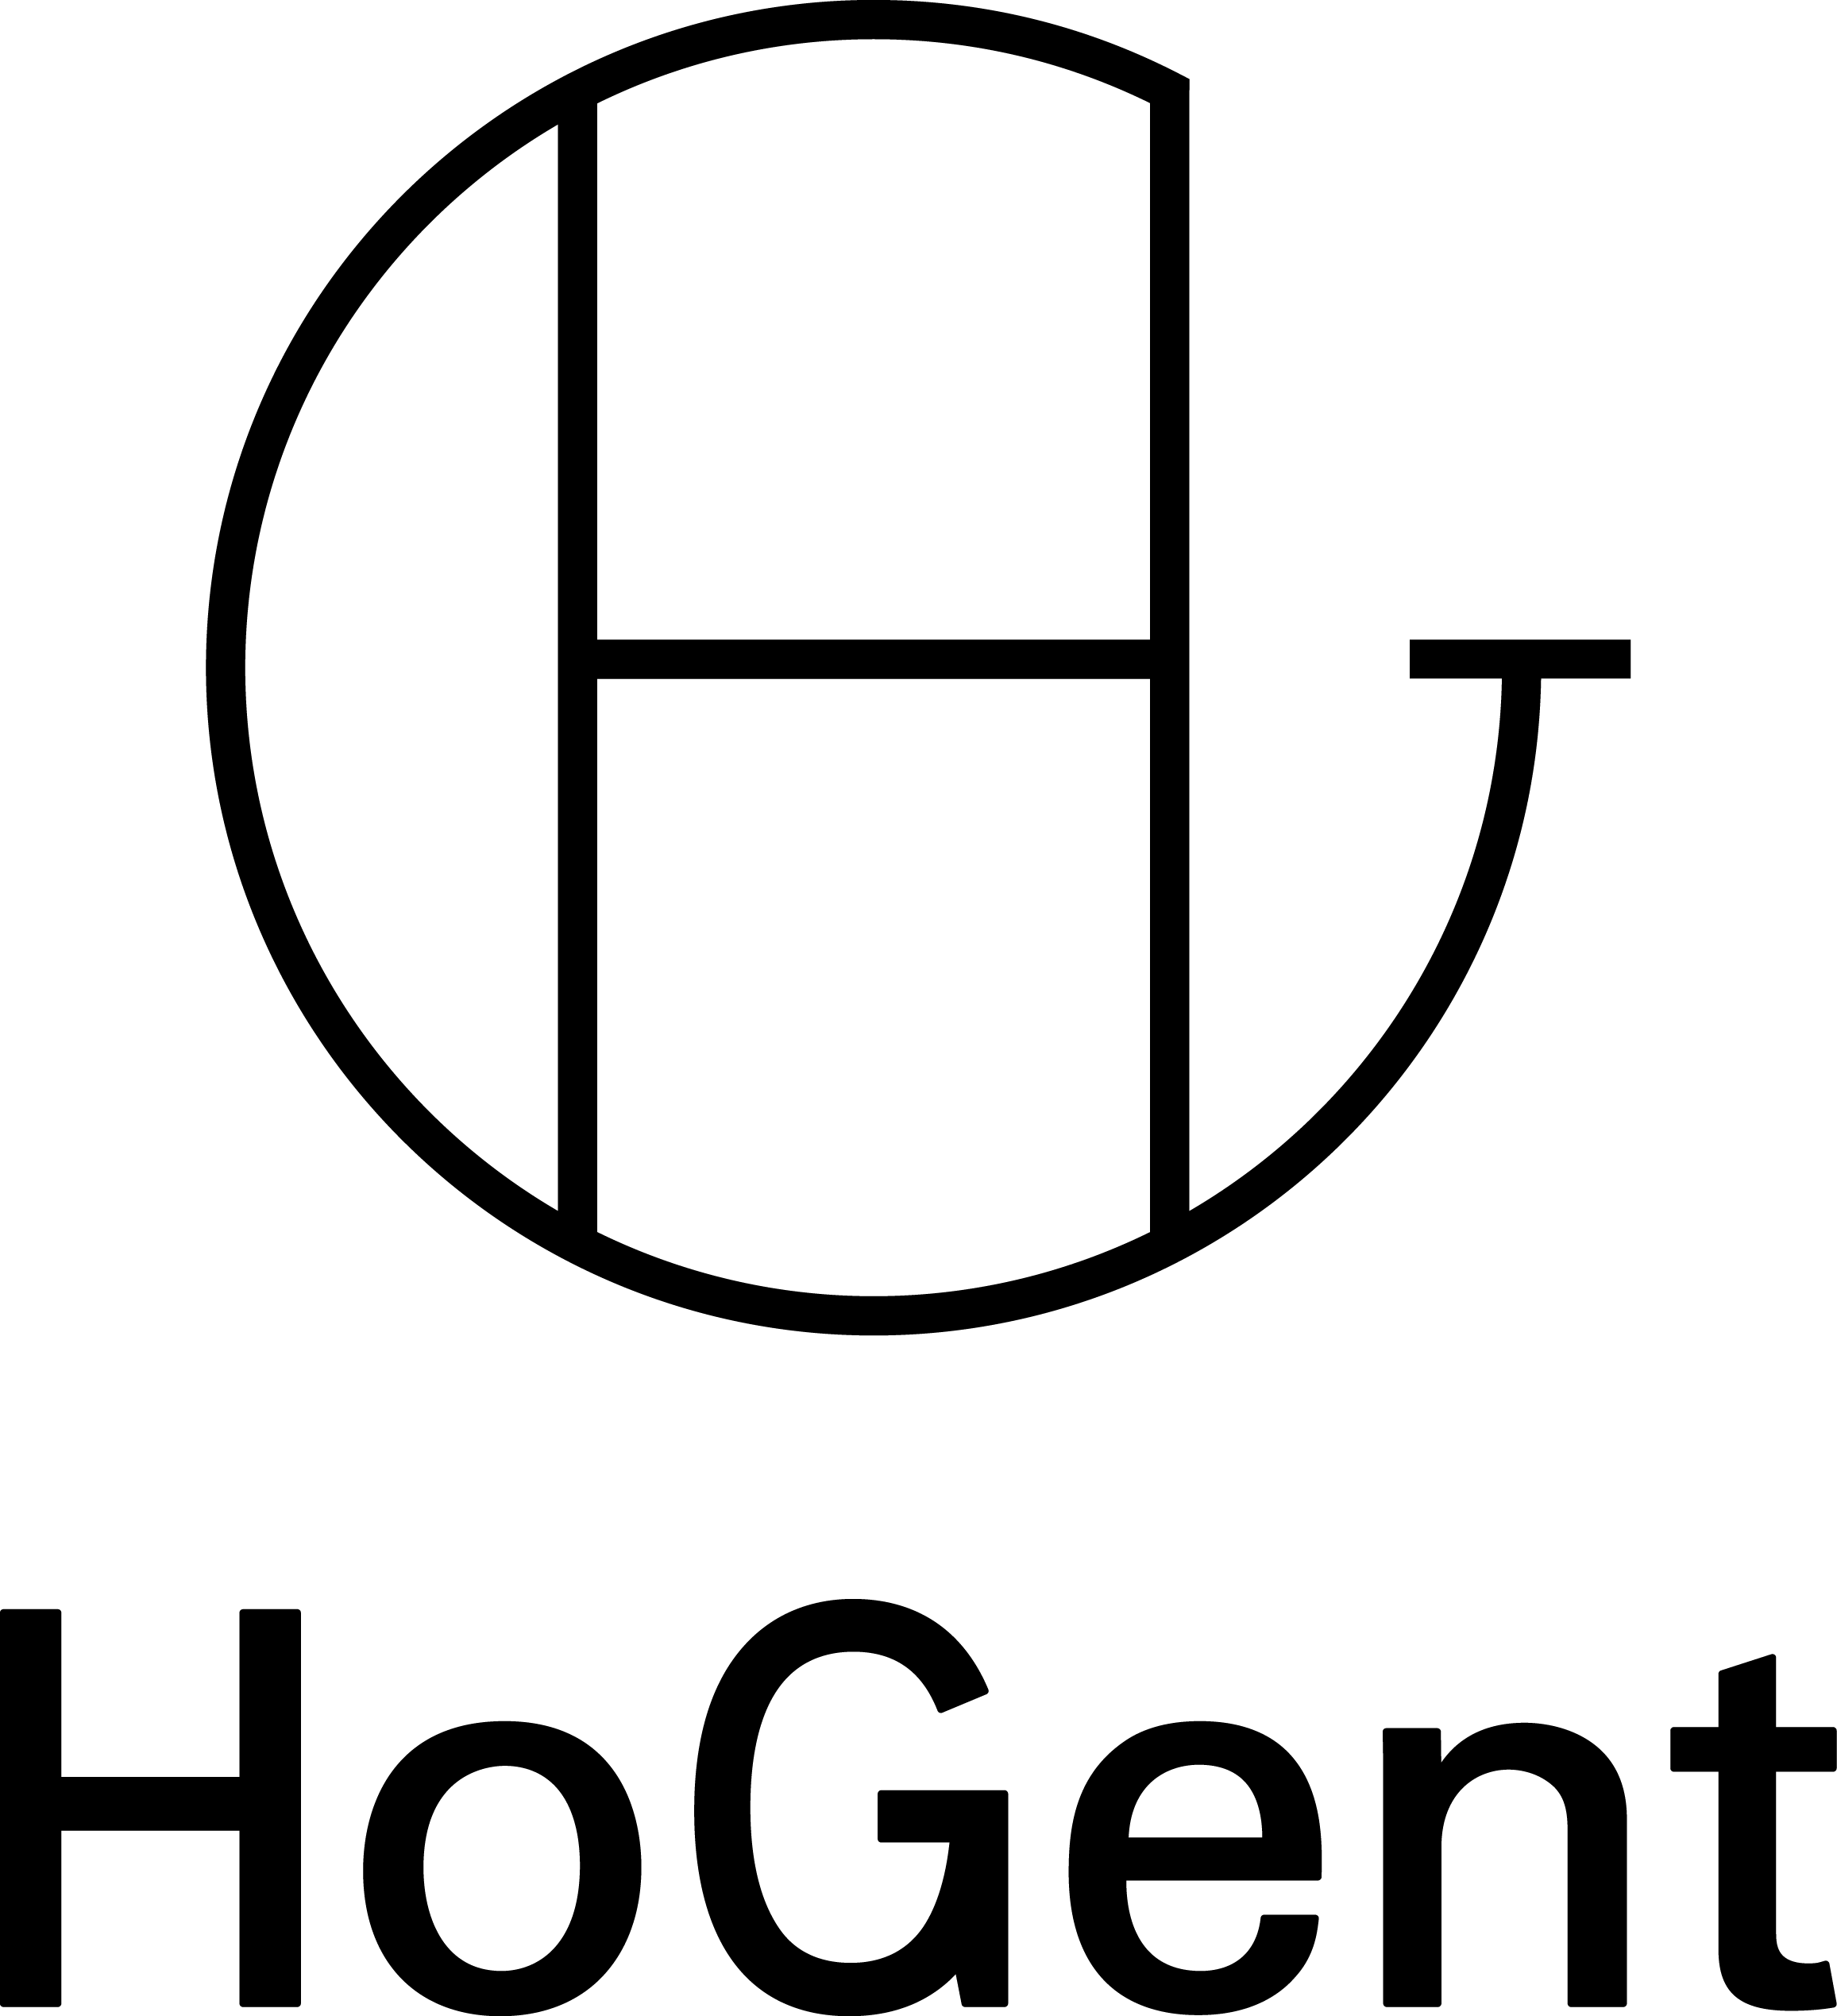
\includegraphics[width=2.5cm]{img/HG-beeldmerk-woordmerk}\\[.5cm]
    Faculteit Bedrijf en Organisatie\\[3cm]
    \titel
    \vfill
    \student\\[3.5cm]
    Scriptie voorgedragen tot het bekomen van de graad van\\professionele bachelor in de toegepaste informatica\\[2cm]
    Promotor:\\
    \promotor\\
    \ifdefempty{\copromotor}{\vspace{2.5cm}}{Co-promotor:\\\copromotor\\[2.5cm]}
    Instelling: \instelling\\[.5cm]
    Academiejaar: \academiejaar\\[.5cm]
    \ifcase \examenperiode \or Eerste \or Tweede \else Derde \fi examenperiode
    \endgroup

  \end{center}
  \restoregeometry
\end{titlepage}
  \emptypage
\begin{titlepage}
  \newgeometry{top=5.35cm,bottom=1.5cm,left=1.5cm,right=1.5cm}
  \begin{center}

    \begingroup
    \rmfamily
    \IfLanguageName{dutch}{Faculteit Bedrijf en Organisatie}{Faculty of Business and Information Management}\\[3cm]
    \titel
    \vfill
    \student\\[3.5cm]
    \IfLanguageName{dutch}{Scriptie voorgedragen tot het bekomen van de graad van\\professionele bachelor in de toegepaste informatica}{Thesis submitted in partial fulfillment of the requirements for the degree of\\professional bachelor of applied computer science}\\[2cm]
    Promotor:\\
    \promotor\\
    \ifdefempty{\copromotor}{\vspace{2.5cm}}{Co-promotor:\\\copromotor\\[2.5cm]}
    \IfLanguageName{dutch}{Instelling}{Institution}: \instelling\\[.5cm]
    \IfLanguageName{dutch}{Academiejaar}{Academic year}: \academiejaar\\[.5cm]
    \IfLanguageName{dutch}{%
    \ifcase \examenperiode \or Eerste \or Tweede \else Derde \fi examenperiode}{%
    \ifcase \examenperiode \or First \or Second \else Third \fi examination period}
    \endgroup

  \end{center}
  \restoregeometry
\end{titlepage}
}

%----------------------------------------------------------------------------------------
%	BIBLIOGRAPHY AND INDEX
%----------------------------------------------------------------------------------------

\usepackage[style=apa,backend=biber]{biblatex}
\usepackage{csquotes}
\DeclareLanguageMapping{dutch}{dutch-apa}
\addbibresource{bachproef-tin.bib} % BibTeX bibliography file
\defbibheading{bibempty}{}

\usepackage{calc} % For simpler calculation - used for spacing the index letter headings correctly
\usepackage{makeidx} % Required to make an index
\makeindex % Tells LaTeX to create the files required for indexing

%----------------------------------------------------------------------------------------
%	MAIN TABLE OF CONTENTS
%----------------------------------------------------------------------------------------

\usepackage{titletoc} % Required for manipulating the table of contents

\contentsmargin{0cm} % Removes the default margin

% Part text styling
\titlecontents{part}[0cm]
{\addvspace{20pt}\centering\large\bfseries}
{}
{}
{}

% Chapter text styling
\titlecontents{chapter}[1.25cm] % Indentation
{\addvspace{12pt}\large\sffamily\bfseries} % Spacing and font options for chapters
{\color{maincolor!60}\contentslabel[\Large\thecontentslabel]{1.25cm}\color{maincolor}} % Chapter number
{\color{maincolor}}
{\color{maincolor!60}\normalsize\;\titlerule*[.5pc]{.}\;\thecontentspage} % Page number

% Section text styling
\titlecontents{section}[1.25cm] % Indentation
{\addvspace{3pt}\sffamily\bfseries} % Spacing and font options for sections
{\contentslabel[\thecontentslabel]{1.25cm}} % Section number
{}
{\hfill\color{black}\thecontentspage} % Page number
[]

% Subsection text styling
\titlecontents{subsection}[1.25cm] % Indentation
{\addvspace{1pt}\sffamily\small} % Spacing and font options for subsections
{\contentslabel[\thecontentslabel]{1.25cm}} % Subsection number
{}
{\ \titlerule*[.5pc]{.}\;\thecontentspage} % Page number
[]

% List of figures
\titlecontents{figure}[0em]
{\addvspace{-5pt}\sffamily}
{\thecontentslabel\hspace*{1em}}
{}
{\ \titlerule*[.5pc]{.}\;\thecontentspage}
[]

% List of tables
\titlecontents{table}[0em]
{\addvspace{-5pt}\sffamily}
{\thecontentslabel\hspace*{1em}}
{}
{\ \titlerule*[.5pc]{.}\;\thecontentspage}
[]

%----------------------------------------------------------------------------------------
%	MINI TABLE OF CONTENTS IN PART HEADS
%----------------------------------------------------------------------------------------

% Chapter text styling
\titlecontents{lchapter}[0em] % Indenting
{\addvspace{15pt}\large\sffamily\bfseries} % Spacing and font options for chapters
{\color{maincolor}\contentslabel[\Large\thecontentslabel]{1.25cm}\color{maincolor}} % Chapter number
{}
{\color{maincolor}\normalsize\sffamily\bfseries\;\titlerule*[.5pc]{.}\;\thecontentspage} % Page number

% Section text styling
\titlecontents{lsection}[0em] % Indenting
{\sffamily\small} % Spacing and font options for sections
{\contentslabel[\thecontentslabel]{1.25cm}} % Section number
{}
{}

% Subsection text styling
\titlecontents{lsubsection}[.5em] % Indentation
{\normalfont\footnotesize\sffamily} % Font settings
{}
{}
{}

%----------------------------------------------------------------------------------------
%	PAGE HEADERS
%----------------------------------------------------------------------------------------

\usepackage{fancyhdr} % Required for header and footer configuration

\pagestyle{fancy}
\renewcommand{\chaptermark}[1]{\markboth{\sffamily\normalsize\bfseries\chaptername\ \thechapter.\ #1}{}} % Chapter text font settings
\renewcommand{\sectionmark}[1]{\markright{\sffamily\normalsize\thesection\hspace{5pt}#1}{}} % Section text font settings
\fancyhf{} \fancyhead[LE,RO]{\sffamily\normalsize\thepage} % Font setting for the page number in the header
\fancyhead[LO]{\rightmark} % Print the nearest section name on the left side of odd pages
\fancyhead[RE]{\leftmark} % Print the current chapter name on the right side of even pages
\renewcommand{\headrulewidth}{0.5pt} % Width of the rule under the header
\addtolength{\headheight}{2.5pt} % Increase the spacing around the header slightly
\renewcommand{\footrulewidth}{0pt} % Removes the rule in the footer
\fancypagestyle{plain}{\fancyhead{}\renewcommand{\headrulewidth}{0pt}} % Style for when a plain pagestyle is specified

% Removes the header from odd empty pages at the end of chapters
\makeatletter
\renewcommand{\cleardoublepage}{
\clearpage\ifodd\c@page\else
\hbox{}
\vspace*{\fill}
\thispagestyle{empty}
\newpage
\fi}

%----------------------------------------------------------------------------------------
%	THEOREM STYLES
%----------------------------------------------------------------------------------------

\usepackage{amsmath,amsfonts,amssymb,amsthm} % For math equations, theorems, symbols, etc

\newcommand{\intoo}[2]{\mathopen{]}#1\,;#2\mathclose{[}}
\newcommand{\ud}{\mathop{\mathrm{{}d}}\mathopen{}}
\newcommand{\intff}[2]{\mathopen{[}#1\,;#2\mathclose{]}}
\newtheorem{notation}{Notation}[chapter]

% Boxed/framed environments
\newtheoremstyle{maincolornumbox}% % Theorem style name
{0pt}% Space above
{0pt}% Space below
{\normalfont}% % Body font
{}% Indent amount
{\small\bf\sffamily\color{maincolor}}% % Theorem head font
{\;}% Punctuation after theorem head
{0.25em}% Space after theorem head
{\small\sffamily\color{maincolor}\thmname{#1}\nobreakspace\thmnumber{\@ifnotempty{#1}{}\@upn{#2}}% Theorem text (e.g. Theorem 2.1)
\thmnote{\nobreakspace\the\thm@notefont\sffamily\bfseries\color{black}---\nobreakspace#3.}} % Optional theorem note
\renewcommand{\qedsymbol}{$\blacksquare$}% Optional qed square

\newtheoremstyle{blacknumex}% Theorem style name
{5pt}% Space above
{5pt}% Space below
{\normalfont}% Body font
{} % Indent amount
{\small\bf\sffamily}% Theorem head font
{\;}% Punctuation after theorem head
{0.25em}% Space after theorem head
{\small\sffamily{\tiny\ensuremath{\blacksquare}}\nobreakspace\thmname{#1}\nobreakspace\thmnumber{\@ifnotempty{#1}{}\@upn{#2}}% Theorem text (e.g. Theorem 2.1)
\thmnote{\nobreakspace\the\thm@notefont\sffamily\bfseries---\nobreakspace#3.}}% Optional theorem note

\newtheoremstyle{blacknumbox} % Theorem style name
{0pt}% Space above
{0pt}% Space below
{\normalfont}% Body font
{}% Indent amount
{\small\bf\sffamily}% Theorem head font
{\;}% Punctuation after theorem head
{0.25em}% Space after theorem head
{\small\sffamily\thmname{#1}\nobreakspace\thmnumber{\@ifnotempty{#1}{}\@upn{#2}}% Theorem text (e.g. Theorem 2.1)
\thmnote{\nobreakspace\the\thm@notefont\sffamily\bfseries---\nobreakspace#3.}}% Optional theorem note

% Non-boxed/non-framed environments
\newtheoremstyle{maincolornum}% % Theorem style name
{5pt}% Space above
{5pt}% Space below
{\normalfont}% % Body font
{}% Indent amount
{\small\bf\sffamily\color{maincolor}}% % Theorem head font
{\;}% Punctuation after theorem head
{0.25em}% Space after theorem head
{\small\sffamily\color{maincolor}\thmname{#1}\nobreakspace\thmnumber{\@ifnotempty{#1}{}\@upn{#2}}% Theorem text (e.g. Theorem 2.1)
\thmnote{\nobreakspace\the\thm@notefont\sffamily\bfseries\color{black}---\nobreakspace#3.}} % Optional theorem note
\renewcommand{\qedsymbol}{$\blacksquare$}% Optional qed square
\makeatother

% Defines the theorem text style for each type of theorem to one of the three styles above
\newcounter{dummy}
\numberwithin{dummy}{section}
\theoremstyle{maincolornumbox}
\newtheorem{theoremeT}[dummy]{Theorem}
\newtheorem{problem}{Problem}[chapter]
\newtheorem{exerciseT}{Exercise}[chapter]
\theoremstyle{blacknumex}
\newtheorem{exampleT}{Example}[chapter]
\theoremstyle{blacknumbox}
\newtheorem{vocabulary}{Vocabulary}[chapter]
\newtheorem{definitionT}{Definition}[section]
\newtheorem{corollaryT}[dummy]{Corollary}
\theoremstyle{maincolornum}
\newtheorem{proposition}[dummy]{Proposition}

%----------------------------------------------------------------------------------------
%	DEFINITION OF COLORED BOXES
%----------------------------------------------------------------------------------------

\RequirePackage[framemethod=default]{mdframed} % Required for creating the theorem, definition, exercise and corollary boxes

% Theorem box
\newmdenv[skipabove=7pt,
skipbelow=7pt,
backgroundcolor=black!5,
linecolor=maincolor,
innerleftmargin=5pt,
innerrightmargin=5pt,
innertopmargin=5pt,
leftmargin=0cm,
rightmargin=0cm,
innerbottommargin=5pt]{tBox}

% Exercise box
\newmdenv[skipabove=7pt,
skipbelow=7pt,
rightline=false,
leftline=true,
topline=false,
bottomline=false,
backgroundcolor=maincolor!10,
linecolor=maincolor,
innerleftmargin=5pt,
innerrightmargin=5pt,
innertopmargin=5pt,
innerbottommargin=5pt,
leftmargin=0cm,
rightmargin=0cm,
linewidth=4pt]{eBox}

% Definition box
\newmdenv[skipabove=7pt,
skipbelow=7pt,
rightline=false,
leftline=true,
topline=false,
bottomline=false,
linecolor=maincolor,
innerleftmargin=5pt,
innerrightmargin=5pt,
innertopmargin=0pt,
leftmargin=0cm,
rightmargin=0cm,
linewidth=4pt,
innerbottommargin=0pt]{dBox}

% Corollary box
\newmdenv[skipabove=7pt,
skipbelow=7pt,
rightline=false,
leftline=true,
topline=false,
bottomline=false,
linecolor=gray,
backgroundcolor=black!5,
innerleftmargin=5pt,
innerrightmargin=5pt,
innertopmargin=5pt,
leftmargin=0cm,
rightmargin=0cm,
linewidth=4pt,
innerbottommargin=5pt]{cBox}

% Creates an environment for each type of theorem and assigns it a theorem text style from the "Theorem Styles" section above and a colored box from above
\newenvironment{theorem}{\begin{tBox}\begin{theoremeT}}{\end{theoremeT}\end{tBox}}
\newenvironment{exercise}{\begin{eBox}\begin{exerciseT}}{\hfill{\color{maincolor}\tiny\ensuremath{\blacksquare}}\end{exerciseT}\end{eBox}}
\newenvironment{definition}{\begin{dBox}\begin{definitionT}}{\end{definitionT}\end{dBox}}
\newenvironment{example}{\begin{exampleT}}{\hfill{\tiny\ensuremath{\blacksquare}}\end{exampleT}}
\newenvironment{corollary}{\begin{cBox}\begin{corollaryT}}{\end{corollaryT}\end{cBox}}

%----------------------------------------------------------------------------------------
%	REMARK ENVIRONMENT
%----------------------------------------------------------------------------------------

\newenvironment{remark}{\par\vspace{10pt}\small % Vertical white space above the remark and smaller font size
\begin{list}{}{
\leftmargin=35pt % Indentation on the left
\rightmargin=25pt}\item\ignorespaces % Indentation on the right
\makebox[-2.5pt]{\begin{tikzpicture}[overlay]
\node[draw=maincolor!60,line width=1pt,circle,fill=maincolor!25,font=\sffamily\bfseries,inner sep=2pt,outer sep=0pt] at (-15pt,0pt){\textcolor{maincolor}{R}};\end{tikzpicture}} % Orange R in a circle
\advance\baselineskip -1pt}{\end{list}\vskip5pt} % Tighter line spacing and white space after remark

%----------------------------------------------------------------------------------------
%	SECTION NUMBERING IN THE MARGIN
%----------------------------------------------------------------------------------------

\makeatletter
\renewcommand{\@seccntformat}[1]{\llap{\textcolor{maincolor}{\csname the#1\endcsname}\hspace{1em}}}
\renewcommand{\section}{\@startsection{section}{1}{\z@}
{-4ex \@plus -1ex \@minus -.4ex}
{1ex \@plus.2ex }
{\normalfont\large\sffamily\bfseries}}
\renewcommand{\subsection}{\@startsection {subsection}{2}{\z@}
{-3ex \@plus -0.1ex \@minus -.4ex}
{0.5ex \@plus.2ex }
{\normalfont\sffamily\bfseries}}
\renewcommand{\subsubsection}{\@startsection {subsubsection}{3}{\z@}
{-2ex \@plus -0.1ex \@minus -.2ex}
{.2ex \@plus.2ex }
{\normalfont\small\sffamily\bfseries}}
\renewcommand\paragraph{\@startsection{paragraph}{4}{\z@}
{-2ex \@plus-.2ex \@minus .2ex}
{.1ex}
{\normalfont\small\sffamily\bfseries}}

%----------------------------------------------------------------------------------------
%	PART HEADINGS
%----------------------------------------------------------------------------------------

% numbered part in the table of contents
\newcommand{\@mypartnumtocformat}[2]{%
\setlength\fboxsep{0pt}%
\noindent\colorbox{maincolor!20}{\strut\parbox[c][.7cm]{\ecart}{\color{maincolor!70}\Large\sffamily\bfseries\centering#1}}\hskip\esp\colorbox{maincolor!40}{\strut\parbox[c][.7cm]{\linewidth-\ecart-\esp}{\Large\sffamily\centering#2}}}%
%%%%%%%%%%%%%%%%%%%%%%%%%%%%%%%%%%
% unnumbered part in the table of contents
\newcommand{\@myparttocformat}[1]{%
\setlength\fboxsep{0pt}%
\noindent\colorbox{maincolor!40}{\strut\parbox[c][.7cm]{\linewidth}{\Large\sffamily\centering#1}}}%
%%%%%%%%%%%%%%%%%%%%%%%%%%%%%%%%%%
\newlength\esp
\setlength\esp{4pt}
\newlength\ecart
\setlength\ecart{1.2cm-\esp}
\newcommand{\thepartimage}{}%
\newcommand{\partimage}[1]{\renewcommand{\thepartimage}{#1}}%
\def\@part[#1]#2{%
\ifnum \c@secnumdepth >-2\relax%
\refstepcounter{part}%
\addcontentsline{toc}{part}{\texorpdfstring{\protect\@mypartnumtocformat{\thepart}{#1}}{\partname~\thepart\ ---\ #1}}
\else%
\addcontentsline{toc}{part}{\texorpdfstring{\protect\@myparttocformat{#1}}{#1}}%
\fi%
\startcontents%
\markboth{}{}%
{\thispagestyle{empty}%
\begin{tikzpicture}[remember picture,overlay]%
\node at (current page.north west){\begin{tikzpicture}[remember picture,overlay]%
\fill[maincolor!20](0cm,0cm) rectangle (\paperwidth,-\paperheight);
\node[anchor=north] at (4cm,-3.25cm){\color{maincolor!40}\fontsize{220}{100}\sffamily\bfseries\@Roman\c@part};
\node[anchor=south east] at (\paperwidth-1cm,-\paperheight+1cm){\parbox[t][][t]{8.5cm}{
\printcontents{l}{0}{\setcounter{tocdepth}{1}}%
}};
\node[anchor=north east] at (\paperwidth-1.5cm,-3.25cm){\parbox[t][][t]{15cm}{\strut\raggedleft\color{white}\fontsize{30}{30}\sffamily\bfseries#2}};
\end{tikzpicture}};
\end{tikzpicture}}%
\@endpart}
\def\@spart#1{%
\startcontents%
\phantomsection
{\thispagestyle{empty}%
\begin{tikzpicture}[remember picture,overlay]%
\node at (current page.north west){\begin{tikzpicture}[remember picture,overlay]%
\fill[maincolor!20](0cm,0cm) rectangle (\paperwidth,-\paperheight);
\node[anchor=north east] at (\paperwidth-1.5cm,-3.25cm){\parbox[t][][t]{15cm}{\strut\raggedleft\color{white}\fontsize{30}{30}\sffamily\bfseries#1}};
\end{tikzpicture}};
\end{tikzpicture}}
\addcontentsline{toc}{part}{\texorpdfstring{%
\setlength\fboxsep{0pt}%
\noindent\protect\colorbox{maincolor!40}{\strut\protect\parbox[c][.7cm]{\linewidth}{\Large\sffamily\protect\centering #1\quad\mbox{}}}}{#1}}%
\@endpart}
\def\@endpart{\vfil\newpage
\if@twoside
\if@openright
\null
\thispagestyle{empty}%
\newpage
\fi
\fi
\if@tempswa
\twocolumn
\fi}

%----------------------------------------------------------------------------------------
%	CHAPTER HEADINGS
%----------------------------------------------------------------------------------------

% A switch to conditionally include a picture, implemented by  Christian Hupfer
\newif\ifusechapterimage
\usechapterimagetrue
\newcommand{\thechapterimage}{}%
\newcommand{\chapterimage}[1]{\ifusechapterimage\renewcommand{\thechapterimage}{#1}\fi}%
\def\@makechapterhead#1{%
{\parindent \z@ \raggedright \normalfont
\ifnum \c@secnumdepth >\m@ne
\if@mainmatter
\begin{tikzpicture}[remember picture,overlay]
\node at (current page.north west)
{\begin{tikzpicture}[remember picture,overlay]
\node[anchor=north west,inner sep=0pt] at (0,0) {\ifusechapterimage\includegraphics[width=\paperwidth]{\thechapterimage}\fi};
\draw[anchor=west] (\Gm@lmargin,-9cm) node [line width=2pt,rounded corners=15pt,draw=maincolor,fill=white,fill opacity=0.5,inner sep=15pt]{\strut\makebox[22cm]{}};
\draw[anchor=west] (\Gm@lmargin+.3cm,-9cm) node {\huge\sffamily\bfseries\color{black}\thechapter. #1\strut};
\end{tikzpicture}};
\end{tikzpicture}
\else
\begin{tikzpicture}[remember picture,overlay]
\node at (current page.north west)
{\begin{tikzpicture}[remember picture,overlay]
\node[anchor=north west,inner sep=0pt] at (0,0) {\ifusechapterimage\includegraphics[width=\paperwidth]{\thechapterimage}\fi};
\draw[anchor=west] (\Gm@lmargin,-9cm) node [line width=2pt,rounded corners=15pt,draw=maincolor,fill=white,fill opacity=0.5,inner sep=15pt]{\strut\makebox[22cm]{}};
\draw[anchor=west] (\Gm@lmargin+.3cm,-9cm) node {\huge\sffamily\bfseries\color{black}#1\strut};
\end{tikzpicture}};
\end{tikzpicture}
\fi\fi\par\vspace*{270\p@}}}

%-------------------------------------------

\def\@makeschapterhead#1{%
\begin{tikzpicture}[remember picture,overlay]
\node at (current page.north west)
{\begin{tikzpicture}[remember picture,overlay]
\node[anchor=north west,inner sep=0pt] at (0,0) {\ifusechapterimage\includegraphics[width=\paperwidth]{\thechapterimage}\fi};
\draw[anchor=west] (\Gm@lmargin,-9cm) node [line width=2pt,rounded corners=15pt,draw=maincolor,fill=white,fill opacity=0.5,inner sep=15pt]{\strut\makebox[22cm]{}};
\draw[anchor=west] (\Gm@lmargin+.3cm,-9cm) node {\huge\sffamily\bfseries\color{black}#1\strut};
\end{tikzpicture}};
\end{tikzpicture}
\par\vspace*{270\p@}}
\makeatother

%----------------------------------------------------------------------------------------
%	HYPERLINKS IN THE DOCUMENTS
%----------------------------------------------------------------------------------------

\usepackage{hyperref}
\hypersetup{hidelinks,backref=true,pagebackref=true,hyperindex=true,colorlinks=false,breaklinks=true,urlcolor= maincolor,bookmarks=true,bookmarksopen=false,pdftitle={Title},pdfauthor={Author}}
\usepackage{bookmark}
\bookmarksetup{
open,
numbered,
addtohook={%
\ifnum\bookmarkget{level}=0 % chapter
\bookmarksetup{bold}%
\fi
\ifnum\bookmarkget{level}=-1 % part
\bookmarksetup{color=maincolor,bold}%
\fi
}
}

%----------------------------------------------------------------------------------------
%	Java source code
%----------------------------------------------------------------------------------------

% Commando voor invoegen Java-broncodebestanden (dank aan Niels Corneille)
% Gebruik:
%   \codefragment{source/MijnKlasse.java}{Uitleg bij de code}
%
% Je kan dit aanpassen aan de taal die je zelf het meeste gebruikt in je
% bachelorproef.
\newcommand{\codefragment}[2]{ \lstset{%
  language=java,
  breaklines=true,
  float=th,
  caption={#2},
  basicstyle=\scriptsize,
  frame=single,
  extendedchars=\true
}
\lstinputlisting{#1}}

% Leeg blad
\newcommand{\emptypage}{%
\newpage
\thispagestyle{empty}
\mbox{}
\newpage
}


%%---------- Documenteigenschappen --------------------------------------------
%% TODO: Vul dit aan met je eigen info:

% Je eigen naam
\newcommand{\student}{Matthias Seghers}

% De naam van je promotor (lector van de opleiding)
\newcommand{\promotor}{Bert Van Vreckem}

% De naam van je co-promotor. Als je promotor ook je opdrachtgever is en je
% dus ook inhoudelijk begeleidt (en enkel dan!), mag je dit leeg laten.
\newcommand{\copromotor}{}

% Indien je bachelorproef in opdracht van/in samenwerking met een bedrijf of
% externe organisatie geschreven is, geef je hier de naam. Zoniet laat je dit
% zoals het is.
\newcommand{\instelling}{---}

% De titel van het rapport/bachelorproef
\newcommand{\titel}{Machine learning met Scala, Phyton en Java in Spark}

% Datum van indienen (gebruik telkens de deadline, ook al geef je eerder af)
\newcommand{\datum}{09 december 2016}

% Academiejaar
\newcommand{\academiejaar}{2016-2017}

% Examenperiode
%  - 1e semester = 1e examenperiode => 1
%  - 2e semester = 2e examenperiode => 2
%  - tweede zit  = 3e examenperiode => 3
\newcommand{\examenperiode}{2}

%%=============================================================================
%% Inhoud document
%%=============================================================================

\begin{document}

%---------- Taalselectie ------------------------------------------------------
%% Als je je bachelorproef in het Engels schrijft, haal dan onderstaande regel
%% uit commentaar. Let op: de tekst op de voorkaft blijft in het Nederlands, en
%% dat is ook de bedoeling!
%\selectlanguage{english}

%---------- Titelblad ---------------------------------------------------------
\inserttitlepage

%---------- Samenvatting, voorwoord -------------------------------------------
\usechapterimagefalse
%%=============================================================================
%% Samenvatting
%%=============================================================================

%% TODO: De "abstract" of samenvatting is een kernachtige (~ 1 blz. voor een
%% thesis) synthese van het document.
%%
%% Deze aspecten moeten zeker aan bod komen:
%% - Context: waarom is dit werk belangrijk?
%% - Nood: waarom moest dit onderzocht worden?
%% - Taak: wat heb je precies gedaan?
%% - Object: wat staat in dit document geschreven?
%% - Resultaat: wat was het resultaat?
%% - Conclusie: wat is/zijn de belangrijkste conclusie(s)?
%% - Perspectief: blijven er nog vragen open die in de toekomst nog kunnen
%%    onderzocht worden? Wat is een mogelijk vervolg voor jouw onderzoek?
%%
%% LET OP! Een samenvatting is GEEN voorwoord!

%%---------- Nederlandse samenvatting -----------------------------------------
%%
%% TODO: Als je je bachelorproef in het Engels schrijft, moet je eerst een
%% Nederlandse samenvatting invoegen. Haal daarvoor onderstaande code uit
%% commentaar.
%% Wie zijn bachelorproef in het Nederlands schrijft, kan dit negeren en heel
%% deze sectie verwijderen.

\IfLanguageName{english}{%
\selectlanguage{dutch}
\chapter*{Samenvatting}
\lipsum[1-4]
\selectlanguage{english}
}{}

%%---------- Samenvatting -----------------------------------------------------
%%
%% De samenvatting in de hoofdtaal van het document

\chapter*{\IfLanguageName{dutch}{Samenvatting}{Abstract}}

%\lipsum[1-4]
Artificiële intelligentie is zich steeds meer en meer aan het ontwikkelen. Grote bedrijven als Google, Facebook, ... zijn daar al volop mee bezig. Maar ook kleinere bedrijven beginnen te experimenteren met machine learning. ToThePoint is zo'n bedrijf. Zij hebben een arcademachine die ze helemaal ombouwen met allerlei nieuwe technologieën in de informatica. Artificiële intelligentie maakt daar deel vanuit. Aan de hand van deze arcademachine wilt ToThePoint tonen aan potentiële klanten tot wat ze allemaal in staat zijn. Wanneer mensen op de arcademachine spelen is het de bedoeling dat er op een schermpje naast de machine een boodschap komt met een voorspelling welk spel de speler speelt. Op basis van verschillende parameters zal het mogelijk zijn die voorspelling te doen. De gebruiker wilt natuurlijk niet te lang wachten op die voorspelling of men wil ook niet Tetris zien verschijnen terwijl ze eigenlijk Mortal Kombat spelen. Daarom is het belangrijk dat een snel maar accuraat algoritme gekozen wordt. Tijdens dit onderzoek gaan we opzoek naar het beste algoritme. Na een vergelijkende studie tussen logistische regressie en support vector machine zal het optimale algoritme gebruikt kunnen worden in de implementatie van de arcademachine. Er bestaan veel verschillende machine learning algoritmen. Een eerste belangrijke stap was dus om twee goede algoritmen te vinden en die uitgebreid te bespreken hoe die in elkaar zitten. Daarna wordt logistische regressie en support vector machine geïmplementeerd met het Accord-framework. De implementatie zal stap voor stap gebeuren. Beginnend met voorspellingen tussen twee spelletjes met twee inputparameters. Om tenslotte te eindigen met vier spelletjes en vijf inputparameters. Het snelste algoritme is logistische regressie. Support vector machine is dan een stuk beter in de juiste voorspellingen. De fouten die een SVM(Support vector machine) maakt zijn ook logisch te verklaren in tegenstelling tot logistische regressie. Logistische regressie maakt bijvoorbeeld fouten tussen Mortal Kombat en Tetris wat eigenlijk totaal verschillende spelletjes zijn. SVM maakt enkel fouten tussen Pacman en Arkanoid wat wel te verstaan is want die spelletjes maken enkel en alleen gebruik van een joystick. Support vector machine heeft gemiddeld 169,4067 ms nodig om een hypothese te vormen, $\pm$ 6 keer zoveel als logistische regressie. Een mens zal dit verschil nooit merken maar de effectieve voorspellingen zal een gebruiker wel onthouden. Daarom krijgt support vector machine de voorkeur om in de arcademachine geïmplementeerd te worden

%%=============================================================================
%% Voorwoord
%%=============================================================================

\chapter*{Voorwoord}
\label{ch:voorwoord}

%% TODO:
%% Het voorwoord is het enige deel van de bachelorproef waar je vanuit je
%% eigen standpunt (``ik-vorm'') mag schrijven. Je kan hier bv. motiveren
%% waarom jij het onderwerp wil bespreken.
%% Vergeet ook niet te bedanken wie je geholpen/gesteund/... heeft



%---------- Inhoudstafel ------------------------------------------------------
\pagestyle{empty} % No headers
\tableofcontents % Print the table of contents itself
\cleardoublepage % Forces the first chapter to start on an odd page so it's on the right
\pagestyle{fancy} % Print headers again

%---------- Lijst afkortingen, termen -----------------------------------------
%% Als je een lijst van afkortingen of termen wil toevoegen, dan hoort die
%% hier thuis. Gebruik bijvoorbeeld de ``glossaries'' package.

%%---------- Kern -------------------------------------------------------------

%%=============================================================================
%% Inleiding
%%=============================================================================

\chapter{Inleiding}
\label{ch:inleiding}

%De inleiding moet de lezer alle nodige informatie verschaffen om het onderwerp te begrijpen zonder nog externe werken te moeten raadplegen \autocite{Pollefliet2011}. Dit is een doorlopende tekst die gebaseerd is op al wat je over het onderwerp gelezen hebt (literatuuronderzoek).

%Je verwijst bij elke bewering die je doet, vakterm die je introduceert, enz. naar je bronnen. In \LaTeX{} kan dat met het commando \texttt{$\backslash${textcite\{\}}} of \texttt{$\backslash${autocite\{\}}}. Als argument van het commando geef je de ``sleutel'' van een ``record'' in een bibliografische databank in het Bib\TeX{}-formaat (een tekstbestand). Als je expliciet naar de auteur verwijst in de zin, gebruik je \texttt{$\backslash${}textcite\{\}}.
%Soms wil je de auteur niet expliciet vernoemen, dan gebruik je \texttt{$\backslash${}autocite\{\}}. Hieronder een voorbeeld van elk.

%\textcite{Knuth1998} schreef een van de standaardwerken over sorteer- en zoekalgoritmen. Experten zijn het erover eens dat cloud computing een interessante opportuniteit vormen, zowel voor gebruikers als voor dienstverleners op vlak van informatietechnologie~\autocite{Creeger2009}.

\section{Stand van zaken}
\label{sec:stand-van-zaken}

%% TODO: deze sectie (die je kan opsplitsen in verschillende secties) bevat je
%% literatuurstudie. Vergeet niet telkens je bronnen te vermelden!


De onderzoeken en technieken om de noden van gebruikers te voorspellen kent de laatste jaren een grote opmars. Google en Facebook zijn dan ook volop bezig met eigen onderzoekscentra en technologieën te ontwikkelen om aan Artificiële Intelligentie te doen. FAIR is de afkorting voor Facebook Artificial Intelligence Research. Er zijn wereldwijd 3 labo's die constant opzoek zijn naar nieuwe mogelijkheden binnen AI (Artificiële Intelligentie). RankBrain is een algoritme van Google die a.d.h.v. artificiële intelligentie de ranking van een bepaalde site op zoekpagina's bepaalt.
De persoonlijke advertenties die Google toont zijn veelal gegenereerd met algoritmes.  Maar ook gerelateerde producten of 'wat jou ook kan interesseren'-lijsten worden dikwijls door machine learning opgemaakt. Tensorflow \autocite{tensorflow} is een open source API ontwikkelt door Google die je uiteraard gratis kan gebruiken om zelf toepassingen met AI te maken. De API is ontwikkeld in Python, deze taal is dan ook een van de veel gebruikte in de data science\autocite{pythonMostPopular}.

In deze bachelorproef zullen er voorspellingen gemaakt worden op een arcademachine (\ref{fig:arcademachine}).
\begin{figure}
	\centering
	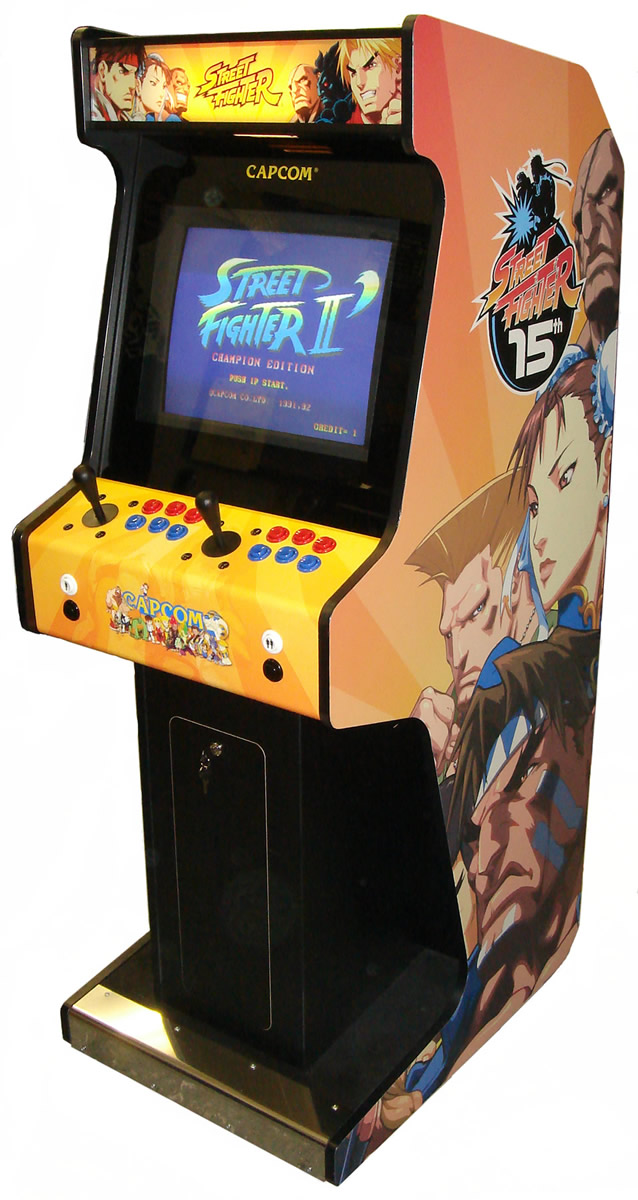
\includegraphics[width=0.6\textwidth]{img/arcademachine}
	\caption{De arcade machine van ToThePoint}
	\label{fig:arcademachine}
\end{figure} ToThePoint zal het eerste bedrijf zijn die AI in een arcademachine zal verwerken. Aangezien er nog geen andere gelijkaardige voorbeelden te vinden zijn zal ervan bij het begin onderzoek gedaan moeten worden. Hoe dit best wordt aangepakt en verklaren waarom. De spelletjes worden bestuurd door zes knoppen en een joystick. Aan de hand van de snelheid van een spel, aantal keer een knop ingedrukt wordt of joystickbeweging is gedaan zullen we kunnen onderscheiden welk spel de gebruiker aan het spelen is. Er bestaan al veel verschillende soorten algoritmen maar deze zijn niet allemaal geschikt voor deze casus en daar zal dus aan gewerkt moeten worden. 

Artificiële intelligentie is hot en zo worden er allerlei beginnende frameworks ontwikkeld die reeds geïmplementeerde algoritmen bevatten of het eenvoudiger maken om ermee te starten. 
Tensorflow is een populair framework ontwikkelt door Google gemaakt in Python. Dit wordt gebruikt in verschillende producten van Google zoals Google's stemherkenning, Google vertaler, het zoeken op afbeeldingen, etc.
TensorFlow maakt gebruik van deep learning-algortimen of neurale netwerken. De voorbeelden van Tensorflow gaan bijna uitsluitend over image recognition maar het is mogelijk om andere applicaties ermee te ontwikkelen. Dit is dan ook de reden dat Google dit framework open source heeft gemaakt zodat ze kunnen zien waar er nog verbeteringen aangebracht kunnen worden en wat er nog allemaal mogelijk is. \autocite{GooglesTensorflow}
Een ander interessant framework is het accord-framework \autocite{accord} die volledig ontwikkeld is in C\#. Hierin zitten veel geïmplementeerde algoritmen die dan kan gebruikt kunnen worden door derden om een eigen applicatie met artificiële intelligentie te ontwikkelen. 

Er zijn al enkele vergelijkingen over algoritmen geweest. Eén daarvan is een vergelijkende studie van verschillende gesuperviseerde algoritmen \autocite{vergelijkingSupervised} Daarin was te vinden dat het support vector machine-algoritme tot de beste gesuperviseerde algoritmen behoort. Doorheen deze bachelorproef zullen we dit algoritme bespreken en vergelijken met logistische regressie. Er is wel vermeld dat de resultaten afhankelijk is van welke dataset gebruikt wordt dus misschien zal in deze casus logistische regressie de voorkeur krijgen.

\section{Probleemstelling en Onderzoeksvragen}
\label{sec:onderzoeksvragen}

%% TODO:
%% Uit je probleemstelling moet duidelijk zijn dat je onderzoek een meerwaarde
%% heeft voor een concrete doelgroep (bv. een bedrijf).
%%
%% Wees zo concreet mogelijk bij het formuleren van je
%% onderzoeksvra(a)g(en). Een onderzoeksvraag is trouwens iets waar nog
%% niemand op dit moment een antwoord heeft (voor zover je kan nagaan).

Machine learning is momenteel aan het boomen. Dit wordt nu zeer veel toegepast voor online advertising met Google en Facebook als de leiders. Maar ook meer en meer bedrijven beginnen zich te verdiepen in artificiële intelligentie. ToThePoint is zich hierop ook aan het voorbereiden. Doormiddel van een funproject willen ze zich zoveel als mogelijk verdiepen in allerlei gebieden binnen de informatica.

Men heeft een arcade machine gekocht die ze volledig gaan customizen met verschillende technologieën. Daar kunnen ze al hun kennis op loslaten. Inclusief de kennis die ze zullen opdoen via deze bachelorproef. Hierdoor zullen ze dus iets bijleren over artificiële intelligentie en dit dan ook kunnen toepassen. Verder zal de machine geplaatst worden op allerlei jobbeurzen om gegevens van studenten op te slaan bijvoorbeeld. Het nut van de machine is niet alleen om bij te leren maar hij zal ook dienen als referentie naar klanten toe. Zo kan ToThePoint aantonen tot wat ze instaat zijn. 

In deze bachelorproef wordt er een vergelijkende studie gemaakt over twee verschillende algoritmen. Het beste algoritme zal dan uiteindelijk geïmplementeerd worden in de arcade machine. Je kan hier heel ver in gaan. De voorspellingen kunnen bijvoorbeeld gemaakt worden door wat de meest gebruikte knop is of joystick beweging. Maar ook door de snelheid dat knoppen bediend worden en de frequentie van dezelfde knop, is het spel eerder een multiplayer spel is of niet,...  aan de hand van deze verschillende factoren is het mogelijk om voorspellingen te doen. Als het nog verder uitgewerkt wordt kan er naar toetsencombinaties gekeken worden maar dit is te vergaand voor deze bachelorproef. Er zal vooral gefocust worden op hoe een goed algoritme gekozen wordt. Het stappenplan die uitgewerkt zal worden kan dan ook toegepast worden op toekomstige projecten. Uiteindelijk zullen we een antwoord hebben op de vraag welk algoritme het meest geschikt is om voorspellingen te doen op een arcademachine.



\section{Opzet van deze bachelorproef}
\label{sec:opzet-bachelorproef}

%% TODO: Het is gebruikelijk aan het einde van de inleiding een overzicht te
%% geven van de opbouw van de rest van de tekst. Deze sectie bevat al een aanzet
%% die je kan aanvullen/aanpassen in functie van je eigen tekst.

De rest van deze bachelorproef is als volgt opgebouwd:

In Hoofdstuk~\ref{ch:methodologie} wordt de methodologie toegelicht en worden de gebruikte onderzoekstechnieken besproken om een antwoord te kunnen formuleren op de onderzoeksvragen.

%% TODO: Vul hier aan voor je eigen hoofstukken, één of twee zinnen per hoofdstuk

In Hoofdstuk~\ref{ch:conclusie}, tenslotte, wordt de conclusie gegeven en een antwoord geformuleerd op de onderzoeksvragen. Daarbij wordt ook een aanzet gegeven voor toekomstig onderzoek binnen dit domein.


%%=============================================================================
%% Methodologie
%%=============================================================================

\chapter{Methodologie}
\label{ch:methodologie}

%% TODO: Hoe ben je te werk gegaan? Verdeel je onderzoek in grote fasen, en
%% licht in elke fase toe welke stappen je gevolgd hebt. Verantwoord waarom je
%% op deze manier te werk gegaan bent. Je moet kunnen aantonen dat je de best
%% mogelijke manier toegepast hebt om een antwoord te vinden op de
%% onderzoeksvraag.


\section{Keuze algoritmen}
\label{sec:keuze-algoritmen}
Om goede resultaten te behalen is het uiterst belangrijk dat de juiste algoritmen gebruikt worden. Zo zijn er bepaalde algoritmen die helemaal niet bruikbaar zouden kunnen zijn voor deze casus. Er zal hier verder uitgelegd worden hoe we een mogelijk algoritme kunnen vinden.

\subsection{Superviseerd vs Ongesuperviseerd leren}
\label{sec: superviseerd-vs-ongesuperviseerd-leren}
Machine learning kan onderverdeelt worden in verschillende types van algoritmen. Deze zijn gesuperviseerd leren, ongesuperviseed leren en reinforcement leren. Dit laatste type is niet van toepassing voor deze casus. Met dit type wordt er geleerd op basis van positieve signalen (beloningen). Er wordt ook niet gebaseerd op een dataset en aangezien wij in bezit zijn van datasets is dit type overbodig om verder te onderzoeken. 

\subsection*{Superviseerd leren}
\label{sec: superviseerd-leren}
Dit type heeft als doel om een hypothese te bekomen die dan zal kunnen gebruikt worden om nieuwe ongekende input toe te wijzen aan een label die voorkwam in de eerdere trainingsdataset. De trainingsdataset bestaat uit verschillende parameters en een label. Onder dit type kan je algoritmen vinden die voor zowat alle cases gebruikt kunnen worden. Deze zijn echter wel nog opgedeeld in drie verschillende categorieën. Zo kan je een nieuwe waarde voorspellen op basis van vroegere resultaten, dit wordt regressie genoemd. Verder heb je classificatiealgoritmen hiermee kan een input toegewezen worden aan een bepaalde klasse met een label. En als laatste bestaan er clusteringsalgoritmen hiermee kan je ook onderverdelingen maken in klassen maar deze hebben geen label. Clustering en classificatie lijken op elkaar maar met classificatie weten we ook precies wat de data voorstelt. 

\subsection*{Ongesuperviseerd leren}
\label{sec: ongesuperviseerd-leren}
Verschillend met gesuperviseerd leren beschikt een ongesuperviseerd algoritme over een ongelabelde dataset. Er zijn verschillende inputs/parameters maar die behoren niet tot een specifieke klasse. Met dit type is het dan ook enkel maar mogelijk om aan clustering te doen. Als we dit willen toepassen voor deze casus is dit geen optimale manier. We kunnen wel bepaalde besturingsevents clusteren waardoor je tot een x aantal clusters kan komen maar we hebben geen idee of de ene cluster PacMan of Mortal Kombat is bijvoorbeeld. 


\textbf{\underline{{\Large misschien een voorbeeldje uitwerken? }}}


\section{Gesuperviseerde classificatie algoritmen}
\label{sec:gesuperviseerde-classificatie-algoritmen}

In deze casus beschikken we over een gelabelde dataset. Het doel is om met een gegeven input een concreet spel te krijgen als output. Doordat we een gelabelde dataset hebben en er verdelingen moeten gemaakt worden op basis van labels is een gesuperviseerd classificatiealgoritme de meest geschikte voor dit onderzoek. Op deze manier kunnen we ongekende input plaatsen bij één bepaald spel.


\subsection{Logistische regressie}
\label{sec:logistische-regressie}

Logistische regressie is het eerste algoritme die we zullen bespreken in deze bachelorproef. Ondanks de naam doet vermoeden, valt dit algoritme niet onder de categorie regressie zoals we in sectie \ref{sec: superviseerd-leren} superviseerd-leren hebben gezien. Dit is wel degelijk een classificatiealgoritme die echter wel gebruik maakt van de logistische functie. Aan de hand van die hypothese kunnen er voorspellingen gemaakt worden. Gedurende het trainingsproces wordt de hypothese geoptimaliseerd. Er zullen meerdere spelletjes voorzien zijn op de arcademachine dus ook meerdere klassen. Omdat we van nul af aan starten zal ook de binaire logistische regressie gebruikt worden en vervolgens zal een van de twee mogelijke methoden om met meerdere klassen te werken gebruikt worden. 

\subsubsection{Binaire logistische regressie}
\label{sec:Binaire-logistische-regressie}

Er moeten enkele puntjes uitgelegd worden voordat we aan de effectieve uitleg kunnen beginnen. Eerst en vooral moeten we weten wat we willen voorspellen. Aangezien we beginnen met binaire logistische regressie maken we een voorspelling tussen twee klassen. Onze vraag kan dus als volgt luiden "Speelt de gebruiker Mortal Kombat of niet?". De waarde \textit{y} zal ons het resultaat geven. \textit{Y} kan slechts twee waarden aannemen $y \; \in \; \{0,1\}$ met 1 als de positieve klasse, Mortal Kombat. Als \textit{y} 0 is dan duidt het op de negatieve klasse, in onze data stelt dit Pacman voor. 

Logistische regressie start vanuit de hypothese van lineaire regressie die als volgt is: 
$$
h(x_{i}) \:= \: \theta^{T}x_{i} \:=\: \theta_{0} \:+ \:\theta_{1}x_{i1} \:+ \: ...\: + \: \theta_{n}x_{in}
$$
$ \theta^{T}$ is de getransponeerde vector van parameters die door het algoritme gegenereerd worden. Als de uitkomst van deze vergelijking $\geq 0$ dan zal de positieve klasse voorspelt worden, de andere klasse zal dan gegeven worden wanneer $h(x) < 0$. 

De logistische regressie is niet meer dan de sigmoïd functie van die lineaire hypothese. Zo krijgen we $h(x) = g(\theta^{T}x)$ . De sigmoïd functie wordt ook wel logistische functie genoemd. Vandaar de naam logistische regressie. 
$$
g(x) \: = \: {\frac{1}{1+e^{-x}}} \: => \: h(x) \: = \:{\frac{1}{1+e^{-\theta^{T}x }}}
$$

De eigenschap van een sigmoïd functie is dat het resultaat altijd zal voldoen aan volgende voorwaarde: $ 0 \leq h(x) \leq1$. 
Nu weten we nog niet wat de waarde van $h(x)$ voor logistische regressie precies uitdrukt. Dit kunnen we wiskundig uitdrukken als $P(y=1|x;\theta)$. M.a.w. de kans dat $y = 1$ voor de gegeven vector \textit{x} met de parameters $\theta$. Wanneer je de kans op de negatieve klasse wenst te weten doet u eenvoudig weg $1 - P(y=1|x;\theta)$. 
\textit{X} kan nu gemakkelijk geclassificeerd worden. Wanneer $h(x)\,\geq\,0.5$ heeft \textit{x} de meeste kans om tot de positieve klasse te behoren in dit geval Mortal Kombat. Anderzijds als $h(x)\:<\:0.5$ zal \textit{x} behoren tot de negatieve klasse. 

\begin{figure}
	\centering
	\begin{tikzpicture} 
	\begin{axis}[
	axis lines = left,
	xlabel = {$\theta^{T}x_{i}$},
	ylabel = {$g(h(\theta^{T}(x))$},
	]
	%Below the red parabola is defined
	\addplot [
	samples=100, 
	color=red,
	]
	{1/(1+exp(-x)};
	%\addlegendentry{$-ln(x)$}
	\end{axis}
	\end{tikzpicture}
	\caption{Sigmoïd functie, wanneer  $\theta^{T}x_{i} = 0$ zal de sigmoïd functie gelijk zijn aan 0.5 dit wil zeggen dat de 2 klassen even veel kans hebben om gekozen te zijn. Naar mate  $\theta^{T}x_{i}$ van waarde verhoogt zal de waarschijnlijkheid voor de positieve klasse ook verhogen. }
	\label{fig:sigmoid-functie}
\end{figure}
 

\subsubsection{Multiklasse logistische regressie}
\label{sec:Multiklasse-logistische-regressie}
Wat u uit de naam al kan afleiden is dat dit een algoritme is om een classificatie te maken over meerdere klassen. Dit kan op twee methoden gedaan worden. De one-vs-one methode of de one-vs-rest(/all) methode. 
\subparagraph{One-vs-all}
Dit is de gemakkelijkste van de twee methoden. Zoals de naam al doet vermoeden vergelijken we één klasse tegenover alle andere klassen. Als er \textit{n} aantal klassen zijn dan zullen er \textit{n} hypothesen $h^{(\,k\,)}$ met $k \in \{\,Pacman, \, Mortal \:Kombat, \, Tetris, \,..\}$ gemaakt worden. \textit{k} is dan de positieve klasse en alle andere klassen samen is dan één negatieve klasse. \newline
Voor een nieuwe input \textit{x} die moet geclassificeerd worden gaat de methode als volgt te werk. $h^{(k)} (x)$ geeft een waarde terug die de waarschijnlijkheid uitdrukt dat x tot de klasse \textit{k} behoort. Dit wordt voor alle \textit{n} hypothesen gedaan. De klasse met de hoogste waarschijnlijkheid wordt dan logischerwijs gekozen als de voorspelde klasse waar \textit{x} toe behoort. 
\subparagraph{One-vs-one}
Met deze techniek vergelijken we twee klassen met elkaar zoals we gezien hebben in sectie \ref{sec:Binaire-logistische-regressie} binaire logistische regressie. Er worden dus opnieuw meerdere hypothesen gemaakt maar anders dan in one-vs-all worden er nu combinaties van twee klassen gebruikt wat er zo uitziet $h^{(\,k,\,m)}$. \textit{k} is in dit geval de positieve klasse en \textit{m} de negatieve. In totaal zullen er $n(n-1)/2$ hypothesen gemaakt worden.
om te bepalen tot welke klasse een nieuwe input \textit{x} behoort berekenen we $h^{(k,m)}(x)$ wanneer het resultaat $\geq 0.5$ krijgt de positieve klasse (\textit{k}) een "punt". Dit gebeurt voor alle hypothesen en de klasse met het meest aantal punten zal uiteindelijk het resultaat zijn van het algoritme. 

\subsubsection{Optimaliseren van algoritme}
\label{sec:Optimaliseren-algoritme}
Om een zo optimaal mogelijk algoritme te verkrijgen moet er gebruik gemaakt worden van optimalisatietechnieken. Gradiënt descent is zo'n techniek die de parameters $\theta$ optimaliseert om een zo'n correct mogelijke hypothese te krijgen. Voordat gradient descent besproken wordt gaan we eerst de kostfunctie bespreken. 

\paragraph{Kostfunctie logistische regressie}
\label{par:kostfunctie-log}
Een kostfunctie wordt genoteerd als $J(\theta)$. Die functie drukt de gemiddelde kost van de trainingsset met parameters $\theta$ uit. Aan de hand van gradient descent is het dan mogelijk om de parameters te optimaliseren zodat de kostfunctie geminimaliseerd wordt. Hoe lager de kostfunctie is hoe beter de hypothese.
De kostfunctie voor logistische regressie ziet er als volgt uit: 
$$ 
J(\theta) \; = \frac{1}{m}\sum_{i=1}^{m} \;   Kost (h_{\theta}(x^{(i)}), y^{(i)} )  
$$

De kost wordt als volgt berekent:
$$Kost (h_{\theta}(x), y) \; = \; -y\ln(h_{\theta}(x)) \;- \;(1-y) \ln(1-h_{\theta}(x))  \;\;\;\; met \; y \in \{0,1\}$$

We stellen \textit{y} gelijk aan 1. Dan zien we dat eigenlijk enkel het eerste deel van de functie ($-y\ln(h_{\theta}(x))$) van belang zal zijn want het tweede deel ($- (1-y) \ln(1-h_{\theta}(x))$ zal nul zijn omdat 1-\textit{y} dan nul zal zijn en dus het product ook nul is. Zo krijgen we: 
\newline $Kost (h_{\theta}(x), y) \; = \; -\ln(h_{\theta}(x))$. Op deze manier komen we uit bij de rode kostfunctie die u ziet in figuur \ref{fig:kostfunctie} p\pageref{fig:kostfunctie}.

$h_{\theta}(x)$ is de hypothese die uitgelegd is in \ref{sec:Binaire-logistische-regressie} binaire logistische regressie. Dus die drukt de waarschijnlijkheid uit dat een vector \textit{x} positief of negatief is. Wanneer we een perfect voorspelling willen dan zou de kost 0 moeten zijn enkel zo ben je volledig zeker dat het label die aan \textit{x} wordt toegekend 100\% positief of negatief is. Als de hypothese zo goed als zeker is dat het vector positief is zal de kost nog dicht bij nul zijn. Eens $h(x) > 0.5$ zal de kost sneller stijgen. Ditzelfde principe geldt voor de negatieve voorbeelden. 

De kostfunctie in één uitdrukking is: 
$$ 
min \;\; -\frac{1}{m}\;\sum_{i=1}^{m} \;  y^{(i)}\ln(h_{\theta}(x^{(i)})) \;- \;(1-y^{(i)}) \ln(1\:-\:h_{\theta}(x^{(i)}))  
$$

Er zijn nog andere kostfuncties die gebruikt kunnen worden maar deze wordt in het algemeen altijd gebruikt.
De functie kan afgeleid worden door een principe binnen statistiek namelijk het 'maximum likelihood estimation'-principe Dit is een manier om parameters te zoeken voor verschillende modellen zoals logistische regressie. Deze functie is ook convex. Convex is een eigenschap die gebruikt wordt voor optimalisatiefuncties. Dit houdt onder meer in dat de functie het globaal minimum bereikt. 

\begin{figure}
	\centering
		\begin{tikzpicture} 
		\begin{axis}[
		axis lines = left,
		xlabel = {$h(x)$},
		ylabel = {$Kost (h_{\theta}(x), y)$},
		]
		%Below the red parabola is defined
		\addplot [
		domain=0:1, 
		samples=100, 
		color=red,
		]
		{-ln(x)};
		\addlegendentry{$-ln(x)$}
		%Here the blue parabloa is defined
		\addplot [
		domain=0:1, 
		samples=100, 
		color=blue,
		]
		{-ln(1-x)};
		\addlegendentry{$-ln(1-x)$}
		
		\end{axis}
		\end{tikzpicture}
	\caption{Visualisatie functies}
	\label{fig:kostfunctie}
\end{figure}

\subsubsection{Gradient descent}
\label{sec:gradient-descent}
Gradient descent is een optimalisatiealgoritme die veel gebruikt wordt voor logistische regressie. Op deze manier is het mogelijk om de parameters $\theta$ te minimaliseren zodat de hypothese goede voorspellingen kan doen.
Gradient descent vereist een continue afleidbare functie, de kostfunctie die we zonet besproken hebben voldoet aan die vereisten. Er is ook een functie \textit{g} nodig die een vector teruggeeft als gradiënt en een stapgrootte $\alpha$. De stapgrootte zorgt ervoor dat het algoritme naar een lokaal of globaal minimum kan convergeren. Wanneer het algoritme stopt in een lokaal minimum heb je niet altijd de beste oplossing tenzij het lokaal minimum ook het globaal minimum is. Indien dit niet het geval is kan gradient descent een aantal keer herhaald worden zodat het globaal minimum kan gevonden worden. Het belang van een goede stapgrootte $\alpha$ is belangrijk. Wanneer die te groot is dan zou het kunnen dat het algoritme in een oneindige lus geraakt. Of als $\alpha$ te klein is dan kan het zeer lang duren tegen dat er een lokaal minimum gevonden is. 

Voor iedere parameter $\theta_{n}$ wordt volgende uitdrukking berekent en terug toegekend aan zichzelf. Tot de parameter amper nog verbetert. In implementaties is het mogelijk om te zeggen dat gradient descent moet stoppen wanneer het verschil van de nieuwe en oude parameter onder een bepaalde grens ligt. 
$$
\theta_{i} = \theta_{i} - \alpha\:\frac{\partial}{\partial\theta_{i}}(J(\theta_{i}, ... , \theta{n}))
$$

Deze functie kan afgeleid worden naar 
$$
\theta_{i} = \theta_{i} - \alpha\:\sum_{i=1}^{m}(h_{\theta}(x^{(i)})\:-\:y^{(i)} ) x_{j}^{(i) }
$$

\textbf{\textit{(Misschien nog voorbeeldje uitwerken en lokaal/globaal minimum uitleggen)}}


\subsection{Support Vector Machine}
\label{sec:Support-Vector-Machine}
Support Vector Machine is een volgend gesuperviseerd leeralgoritme die zal besproken worden. 
Andrew Ng is professor aan de Stanford University begon het deel support vectormachine in zijn cursus \autocite{cursusAndrewNg} met volgende zin.
\begin{quote}
	SVMs are among the best (and many believe are indeed the best) ‘off-the-shelf’ supervised learning algorithms.
\end{quote}

SVMs scoren over het algemeen beter dan logistische regressie of neurale netwerken. Het is uiteraard mogelijk dat een van die twee beter scoort maar dit is allemaal afhankelijk van de dataset. Vandaar dat het een logische keuze is om dit algoritme te vergelijken met ons vorige, logistische regressie. 

We maken gebruik van figuur \ref{fig:svm} op pagina \pageref{fig:svm} om de werking van een SVM uit te leggen. Daarna zal de kostfunctie uitgelegd worden die gebruikt wordt om het algoritme te optimaliseren. Dit alles is vereenvoudigd zodat het al mens makkelijker in te beelden is.
Het concept van SVM klinkt eenvoudig. De bedoeling is om een hyperplane te vinden die tussen de dichtstbijzijnde vector van een klasse en de hyperplane een zo groot mogelijke marge heeft. U ziet in de figuur dat het mogelijk is om meerdere hyperplanes te tekenen maar niet iedere hyperplane heeft een even grote marge. Om de marge beter te begrijpen gaan we eventjes terug naar logistische regressie. Daar kregen we een waarschijnlijkheid dat vector \textit{x} van een bepaalde klasse is. Als $\theta^{T}x \geq 0$ was $y=1$ en vice versa. Het is logisch dat hoe verder $\theta^{T}x$ van 0 ligt hoe zekerder de klasse kan toegekend worden. Dit is net wat SVM bijbrengt, een marge zodat je vanaf een bepaalde zekerheid, marge, pas een klasse toekent. Een marge wiskundige noteren is als volgt: $\theta^{T}x^{i} \ll 0$. $\ll$ betekent veel minder. Deze uitdrukking geldt dus voor $y^{i}=0$
 
Eerst en vooral wordt er een hyperplane gezocht die twee klassen van elkaar onderscheid. Zoals je in de figuur ziet is het mogelijk om meerdere hyperplanes (A,B) te maken. Die hyperplanes zijn van de vorm $h_{w,b}(x) = w^{T}x + b$ $w$ stelt nu $\theta_{n}^{T}$ voor en $b$ stelt $\theta_{0}$ voor. \textit{y} is nu geen element meer van {0,1} maar wel van {1,-1}. Als $h_{w,b}(x) > 1$ dan kunnen we stellen dat voor vector x een positieve klasse kan voorspelt worden. 
We nemen nu hyperplane \textit{A} om verder op te bouwen. We weten ook dat \textit{A1} het functie voorschrijft $w x +b=1$ heeft en \textit{A2} dan  $w x +b=-1$. Op deze manier is het mogelijk om de marge tussen \textit{A1} en \textit{A2} te berekenen. En die dus te optimaliseren.

\begin{figure}[]
	\centering
	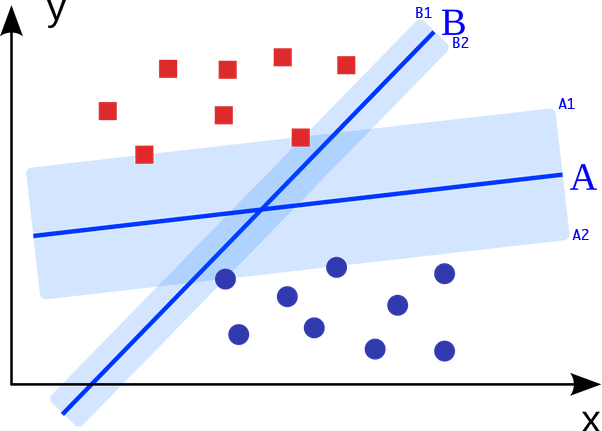
\includegraphics[width=0.6\textwidth]{img/svmkopie}
	\caption{Begeleidende afbeelding SVM \autocite{svmGraph}}
	\label{fig:svm}
\end{figure}

\subsubsection{Kostfunctie Support Vector Machine}

De kostfunctie van een SVM is gelijkaardig als de kostfunctie van logistische regressie. Er zijn enkele verschillen. Hier ziet u nog eens deze van logistische regressie: 
$$ 
min \;\; -\frac{1}{m}\sum_{i=1}^{m} \;  y^{(i)}\ln(h_{\theta}(x^{(i)})) \;- \;(1-y^{(i)}) \ln(1-h_{\theta}(x^{(i)}))  
$$
en de kostfunctie van een support vector machine is: 
$$ 
min \;\; C\sum_{i=1}^{m} \; \left[ y^{(i)}\;cost_{1}(\theta^{T}(x^{(i)})) \;- \;(1-y^{(i)})\;cost_{0}(\theta^{T}\:(x^{(i)})) \right] 
$$

Er zijn 2 grote wijzigingen. Het gedeelte $\ln(h_{\theta}\:(x^{(i)}))$ en $\ln(1-h_{\theta}\:(x^{(i)}))$ zijn vervangen door respectievelijk $cost_{1}\:(\theta^{T}\:(x^{(i)}))$ en $cost_{0}\:(\theta^{T}\:(x^{(i)})) $ 
Die kost functies kan u zien in figuren \ref{fig:cost1} en \ref{fig:cost0}. Als u de functies bekijkt zie u dat er eerst een plat stuk is en dan pas vanaf 1 of -1 begint te stijgen. Dit komt door de marge die we eerder besproken hebben. Wanneer  $\theta^{T}\:(x^{(i)}) \geq 1$ dan kunnen we ervan uit gaan dat $y=1$.
\begin{figure}
	\centering
	\begin{minipage}{.5\textwidth}
		\centering
		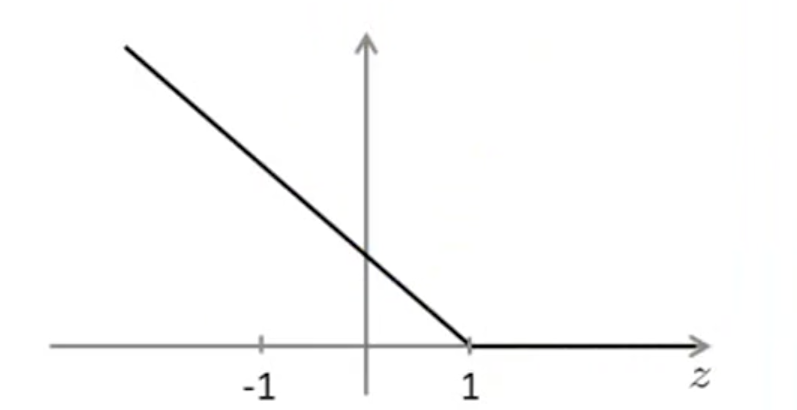
\includegraphics[width=1\linewidth]{img/costEen}
		\caption{$cost_{1}\:(\theta^{T}(x^{(i)}))$}
		\label{fig:cost1}
	\end{minipage}%
	\begin{minipage}{.5\textwidth}
		\centering
		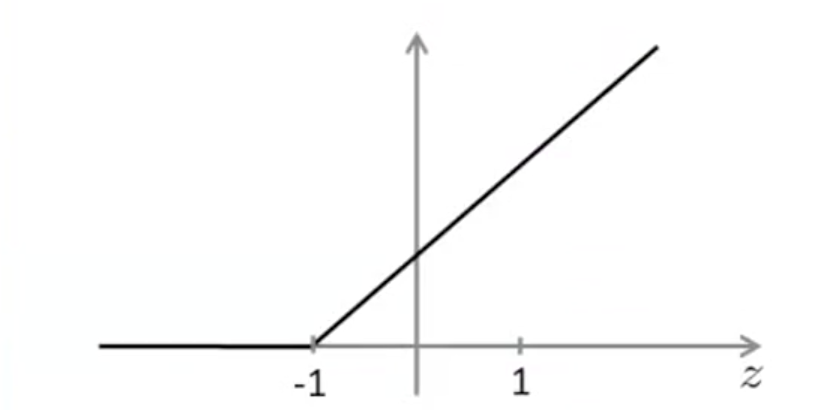
\includegraphics[width=1\linewidth]{img/costNul}
		\caption{$cost_{0}\:(\theta^{T}(x^{(i)})) $}
		\label{fig:cost0}
	\end{minipage}
\end{figure}


\subsection{Selectiecriteria}
\label{sec:Selectiecriteria}
Hoe weten we nu welk algoritme het best is om voorspellingen te doen op de arcade machine? We bespreken enkele selectiecriteria zodat de 2 algoritmen die we zonet besproken hebben kunnen vergelijken. 
Er zijn twee belangrijke factoren die beslissen of dat het ene algoritme beter is dan het andere voor een bepaalde dataset. 
Als we de algoritmen gaan implementeren dan zal altijd exact dezelfde dataset en testset gebruikt worden. De algoritmen worden beiden geïmplementeerd in Visual Studio 2015 en worden gerund zonder dat er een ander programma openstaat of draait in de achtergrond. Tussen de test wordt er ook nooit een ander programma geopend want het is altijd mogelijk dat die daarna nog in de achtergrond processen uitvoert. 

\subsubsection{Snelheid}
Snelheid is uiteraard een van de belangrijkste voorwaarden om een goed algoritme te zijn. Je wilt bijvoorbeeld geen 2 minuten wachten tegen dat je krijgt te weten wat de computer dacht dat je aan het spelen was. Een programma bestaat uit verschillende delen. Niet alle onderdelen van een programma zijn relevant voor deze bachelorproef. Zo heb je bijvoorbeeld het inlezen van de data. Dit proces zal even veel tijd in beslag nemen voor logistische regressie als voor vector support machine doordat dezelfde data gebruikt wordt voor beiden. Een tweede deel is natuurlijk de declaratie van variabelen en objecten dit gebeurt zodanig snel dat dit irrelevant is.\newline
Dan heb je het leerproces of optimalisatieproces van een algoritme. Dit is wel belangrijk want hiermee kan het verschil gemaakt worden. Daarvoor gebruiken we de klasse Stopwatch die in het .NET framework voorzien is. Die wordt gestart net voor de start van het leerproces en gestopt net erna. Op deze manier kunnen we precies meten hoelang het algoritme nodig heeft om een hypothese op te stellen. \newline
We hebben ook nog een gedeelte waar we een nieuwe vector laten voorspellen maar ook dit is enkel maar een wiskundige berekening wat voor de computer praktisch niets inhoudt. 

\subsubsection{F-score}
\label{sec:fscore}
Om een idee te hebben hoe goed een algoritme voorspellingen doet kan je een simpele test doen en kijken hoeveel procent van de testdataset correct werd voorspelt. Er is echter een manier om nog correcter weer te geven hoe goed een algoritme effectief is. Dit kan aan de hand van de F-score. \newline
Wanneer een algoritme een voorspelling doet zijn er vier mogelijke uitkomsten onderverdeelt. Hieronder ziet u de correcte en foute resultaten:
\begin{itemize}
	\item Correcte voorspellingen
	\begin{itemize}
		\item Positieve voorspelling voor een positieve uitkomst  (A)
		\item Negatieve voorspelling voor een negatieve uitkomst (B)
	\end{itemize}
	\item Foutieve voorspellingen
	\begin{itemize}
		\item Positieve voorspelling terwijl de uitkomst negatief had moeten zijn (C)
		\item Negatieve voorspelling terwijl de uitkomst positief had moeten zijn (D)
	\end{itemize}
\end{itemize}

Om de F-score te begrijpen moeten er nog 2 begrippen uitgelegd worden. Als eerste zullen we beginnen met precisie. \newline 
Als je de effectieve juiste positieve voorspelling ($\:$A$\:$) deelt door het totaal aantal positieve voorspelling (dus inclusief positieve voorspellingen van de hypothese maar die eigenlijk negatief had moeten zijn). Dan bekom je een percentage die de precisie uitdrukt. $$precisie\:=\:\frac{A}{A\:+\:C}$$

Rappel is een tweede begrip die eveneens een percentage uitdrukt. Dan wil je weten van alle positieve voorbeelden in de dataset ($\:$A$\:$+$\:$D$\:$) hoeveel de hypothese ook als positief heeft teruggegeven ($\:$A$\:$). $$rappel\:=\: \frac{A}{A\:+\:D}$$

Precisie en rappel zullen dus altijd gelijk aan 1 zijn wanneer het algoritme alle testvoorbeelden het correcte label heeft gegeven. Stel dat een algoritme alle voorbeelden negatief labelt dan zal de rappel gelijk zijn aan 0 ($\frac{0}{0\:+\:D}=0$). Voor precisie geldt het omgekeerde.
De uiteindelijke formule voor de F-score is als volgt: 
$$F-score\:=\: \frac{2* precisie * rappel}{precisie\:+\:rappel}$$
De F-score zal altijd tussen 0 en 1 liggen. Hoe hoger de score hoe beter het algoritme is. 



%% Voeg hier je eigen hoofdstukken toe die de ``corpus'' van je bachelorproef
%% vormen. De structuur en titels hangen af van je eigen onderzoek. Je kan bv.
%% elke fase in je onderzoek in een apart hoofdstuk bespreken.

%\input{}
%\input{}
%...

%%=============================================================================
%% Conclusie
%%=============================================================================

\chapter{Conclusie}
\label{ch:conclusie}

%% TODO: Trek een duidelijke conclusie, in de vorm van een antwoord op de
%% onderzoeksvra(a)g(en). Wat was jouw bijdrage aan het onderzoeksdomein en
%% hoe biedt dit meerwaarde aan het vakgebied/doelgroep? Reflecteer kritisch
%% over het resultaat. Had je deze uitkomst verwacht? Zijn er zaken die nog
%% niet duidelijk zijn? Heeft het ondezoek geleid tot nieuwe vragen die
%% uitnodigen tot verder onderzoek?

%\lipsum[76-80]



%%---------- Back matter ------------------------------------------------------

\printbibliography
\addcontentsline{toc}{chapter}{\textcolor{maincolor}{\IfLanguageName{dutch}{Bibliografie}{Bibliography}}}


\listoffigures
\listoftables

\end{document}
